% This is "sig-alternate.tex" V2.0 May 2012
% This file should be compiled with V2.5 of "sig-alternate.cls" May 2012
%
% This example file demonstrates the use of the 'sig-alternate.cls'
% V2.5 LaTeX2e document class file. It is for those submitting
% articles to ACM Conference Proceedings WHO DO NOT WISH TO
% STRICTLY ADHERE TO THE SIGS (PUBS-BOARD-ENDORSED) STYLE.
% The 'sig-alternate.cls' file will produce a similar-looking,
% albeit, 'tighter' paper resulting in, invariably, fewer pages.
%
% ----------------------------------------------------------------------------------------------------------------
% This .tex file (and associated .cls V2.5) produces:
%       1) The Permission Statement
%       2) The Conference (location) Info information
%       3) The Copyright Line with ACM data
%       4) NO page numbers
%
% as against the acm_proc_article-sp.cls file which
% DOES NOT produce 1) thru' 3) above.
%
% Using 'sig-alternate.cls' you have control, however, from within
% the source .tex file, over both the CopyrightYear
% (defaulted to 200X) and the ACM Copyright Data
% (defaulted to X-XXXXX-XX-X/XX/XX).
% e.g.
% \CopyrightYear{2007} will cause 2007 to appear in the copyright line.
% \crdata{0-12345-67-8/90/12} will cause 0-12345-67-8/90/12 to appear in the copyright line.
%
% ---------------------------------------------------------------------------------------------------------------
% This .tex source is an example which *does* use
% the .bib file (from which the .bbl file % is produced).
% REMEMBER HOWEVER: After having produced the .bbl file,
% and prior to final submission, you *NEED* to 'insert'
% your .bbl file into your source .tex file so as to provide
% ONE 'self-contained' source file.
%
% ================= IF YOU HAVE QUESTIONS =======================
% Questions regarding the SIGS styles, SIGS policies and
% procedures, Conferences etc. should be sent to
% Adrienne Griscti (griscti@acm.org)
%
% Technical questions _only_ to
% Gerald Murray (murray@hq.acm.org)
% ===============================================================
%
% For tracking purposes - this is V2.0 - May 2012

\documentclass{sig-alternate}

\usepackage{listings,xcolor,bera}
\usepackage{graphicx}
%% \usepackage{afterpage}

\colorlet{punct}{red!60!black}
\definecolor{background}{HTML}{EEEEEE}
\definecolor{delim}{RGB}{20,105,176}
\colorlet{numb}{magenta!60!black}

\lstdefinelanguage{json}{
    basicstyle=\normalfont\ttfamily,
    numbers=left,
    numberstyle=\scriptsize,
    stepnumber=1,
    numbersep=8pt,
    showstringspaces=false,
    breaklines=true,
    frame=lines,
    %% backgroundcolor=\color{background},
    literate=
     *{0}{{{\color{numb}0}}}{1}
      {1}{{{\color{numb}1}}}{1}
      {2}{{{\color{numb}2}}}{1}
      {3}{{{\color{numb}3}}}{1}
      {4}{{{\color{numb}4}}}{1}
      {5}{{{\color{numb}5}}}{1}
      {6}{{{\color{numb}6}}}{1}
      {7}{{{\color{numb}7}}}{1}
      {8}{{{\color{numb}8}}}{1}
      {9}{{{\color{numb}9}}}{1}
      {:}{{{\color{punct}{:}}}}{1}
      {,}{{{\color{punct}{,}}}}{1}
      {\{}{{{\color{delim}{\{}}}}{1}
      {\}}{{{\color{delim}{\}}}}}{1}
      {[}{{{\color{delim}{[}}}}{1}
      {]}{{{\color{delim}{]}}}}{1},
}

\begin{document}

\makeatletter
\def\@copyrightspace{\relax}
\makeatother

\title{
Duck - Yet Another Software Visualization Tool to Speed Up Source Codes Understanding
}
%\subtitle{https://github.com/Stumble/duck}

\numberofauthors{5} %  in this sample file, there are a *total*
% of EIGHT authors. SIX appear on the 'first-page' (for formatting
% reasons) and the remaining two appear in the \additionalauthors section.
%
\author{
% You can go ahead and credit any number of authors here,
% e.g. one 'row of three' or two rows (consisting of one row of three
% and a second row of one, two or three).
%
% The command \alignauthor (no curly braces needed) should
% precede each author name, affiliation/snail-mail address and
% e-mail address. Additionally, tag each line of
% affiliation/address with \affaddr, and tag the
% e-mail address with \email.
%
% 1st. author
\alignauthor
Shan He\\
       \affaddr{504774265}\\
       \email{shanhex@gmail.com}
% 2st. author
\alignauthor
Yukai Tu\\
       \affaddr{204761085}\\
       \email{tuyukai1994@gmail.com}
% 3st. author
\alignauthor
Yuling Liu\\
       \affaddr{504777221}\\
       \email{lylwill@ucla.edu}
\and
% 4st. author
\alignauthor
Yumin Xia\\
       \affaddr{404775675}\\
       \email{yumin@cs.ucla.edu}
% 5st. author
\alignauthor
Cong Peng\\
       \affaddr{904760493}\\
       \email{pengcong@ucla.edu}
}

\maketitle
\begin{abstract}
Understanding a software system from scratch is one of the major problems for most software developers. Specifically, it is often difficult to tell which class is of the greatest importance to look at from the very beginning. Thus, we designed and implemented a language independent, interactive software visualization analysis tool called DUCK which can relieve the pressure of understanding an unfamiliar codebase. The DUCK supports multi-metrics measurement compare to some old visualization tools, and it employs interactive visualization figure, Query-able visualization together with application of data mining techniques on metrics to make it a powerful visualization tool. 

\end{abstract}

\section{Introduction}

Nowadays, as codebases grow larger, software systems are one of the most complex and difficult systems to understand.
Meanwhile, reading source codes and understanding key modules are time-consuming prerequisites for the following software development.
To speed up this process, software visualization technique is proposed to be an efficient technique
to facilitate source code understanding, because visual displays allow human brain to study
multiple aspects of complex problems in parallel \cite{petre1995looking}.
Moreover, developers can form an initial picture of the system through visualized diagram \cite{lanza2003object}
and even veteran programmers find it useful \cite{kim2012field}. 

However, visualization technique has downsides.
Firstly, they are usually measured in a single degree,
hard to scale up and lack of visual cues for the viewer to correctly interpret them \cite{fenton2014software}.
To overcome the single degree measurement, \cite{lanza2003polymetric} presents a visual approach that captures multiple software metrics,
like lines of code, method overridden ratio and number of state variable etc.,
linked up associatively, in a single diagram,
to help to understand the structure in an initial phase.
As an enhancement of \cite{lanza2003polymetric}, we have implement following novel features:
\vspace{-2pt}
\begin{enumerate}
  \item \emph{Interactive visualization figure.} The first dynamic feature we provide is that we plot interactive figures as visualization result. User can zoom-in/zoom-out into elements to read the details while having a global view of the whole source codebase. This could address the visualization scalability issue to some degree. 
  \vspace{-6pt}
  \item \emph{Query-able visualization.} The second dynamic feature is that user can explicitly specify what portion of classes he wants to plot. For example, when they want to produce figures related to class C, including its related classes, or when they want to debug on class C. This feature is a true cure to the scalability issue of visualization technique. Our evaluation results show that raters found this feature amazingly useful.
  \vspace{-6pt}
  \item \emph{Application of data mining techniques on metrics.} For example, by applying the PageRank algorithm on class usage dependency graph, we can evaluate the importance of classes from a fresh view. As illustrated in the PageRank implementation section.
\end{enumerate}
\vspace{-2pt}
To summarize, we propose a language independent, interactive, scalable software visualization analysis tool called DUCK, which supports presenting polymetric views of source code, combined with interactive dynamic figure, query-able visualization, and metrics from data mining techniques.

\section{Related Work}
When developers who first look at an unfamiliar code base, it is usually hard to get an overall picture of the whole system.
\cite{stasko1998software} presents some basic ideas on how to build a mental model during software exploration,
but do not provide the much-needed, yet difficult to obtain, empirical evidence.
Lanza, M., and Ducasse, S in \cite{lanza2003polymetric} settled on the following goals for getting a first impression and a mental model of a system:
\vspace{-2pt}
\begin{enumerate}
\item code base size, complexity, structure.
\vspace{-6pt}
\item understand the most important classes and inheritance hierarchies.
\vspace{-6pt}
\item Identify exceptional classes in terms of size and/or complexity.
\vspace{-6pt}
\item Identify the possible presence of design patterns.
\end{enumerate}
\vspace{-2pt}
To get above information from a code base, in the wide array of possible metrics,
we plan to selected the design metrics, which can be extracted from the source code entities themselves.
The metrics we use are termed direct measurement metrics, also include parts of indirect measurement \cite{storey1999cognitive}.

Since software visualizations are often too simplistic and lack visual cues for the viewer to correctly interpret them \cite{petre1995looking},
the most common way is to increase the dimension of the graphs, like concretization and polymetric.
Not only increase the dimension from 2D to 3D, the Codecity also concretize a code base into a city model \cite{wettel2008codecity}.
The buildings in the city represent classes, while the districts represent the software packages.
The CodeCity supports both linear mapping and non-linear mapping for metrics and uses containment-based layout to
display the nesting level of package in each district. In another way, the polymetric try
to present multiple corresponding information within different polymetric layouts \cite{lanza2003polymetric, lanza2005codecrawler, lanza2003object}.
In \cite{lanza2003object}, page 21, it defines the layout types include: Tree, Scatterplot, Histogram, Checker, Stapled, etc.
An implementation of this visualization tool can be found at this website \footnote{http://www.softviscollection.org/polymetric-views/public/polymetrics.html},
which can generate 6 layout graphs in real-time.
We also analyzed another widely used software visualization tool, Moose. Moose is a platform for expressing analyses of software systems and of data in general. Its main goal is to assist and enable a human in the process of understanding large amounts of data.
Aside from Moose, we also investigated on other related software visualization tools, such as Seesoft \cite{eick1992seesoft} and sv3D \cite{maletic2003source}.

Erick and coworkers introduced a new technique for visualizing line oriented statistics associated with source code and a software tool, Seesoft, embodying the technique. There are four key ideas: reduced representation, coloring by statistic, direct manipulation, and capability to read actual code. The reduced representation is achieved by displaying files as columns and lines of code as thin rows within the columns. The color of each row is determined by a statistic associated with the lines of code that it represents. However, their visualization technique provides a qualitative view of the distribution of a statistic in code. As with all graphical methods, the technique is useful for discovering patterns. After the patterns are discovered, hypotheses may be tested by means of standard statistical methods. Currently, Seesoft is unable to display more than 50,000 lines of code simultaneously. A key idea in Seesoft is its interactive use of direct manipulation techniques and use of color. It is difficult to describe these in a static monochrome medium. 

Source Viewer 3D (sv3D) is a software visualization framework that uses a 3D metaphor to represent software system and analysis data. The 3D representation is based on the SeeSoft pixel metaphor. It extends the original metaphor by rendering the visualization in a 3D space. New, object-based manipulation methods and simultaneous alternative mappings are available to the user. sv3D is implemented in C++ and uses Qt for the user interfaces and Open Inventor for 3D rendering. 

In our project, we not only re-implement the previous work, but also improve the metrics and visualization result.
In metrics, we introduce the dynamic supervision on variables, methods, and classes runtime behavior.
As for visualization output, we achieve a more intuitive, more efficient graphical representation.

\begin{figure*}
\centering
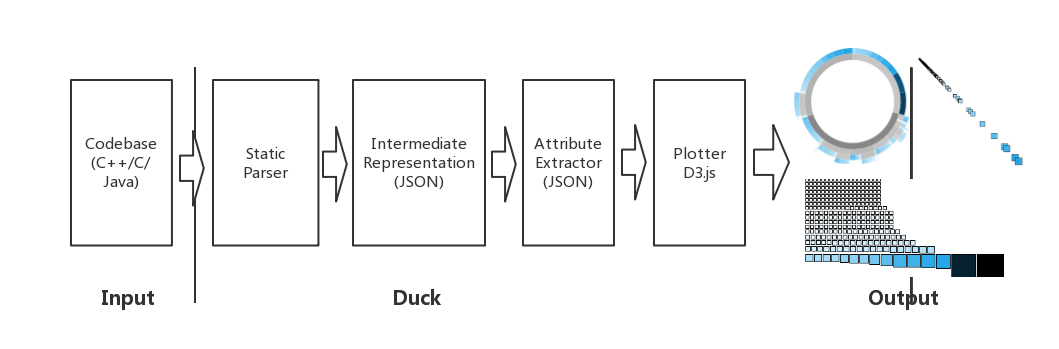
\includegraphics[width=1.0\textwidth]{arch.png}
\caption{Architecture of DUCK}
\label{fig:arch}
\end{figure*}

\section{Approach Description}
To implement this tool, we use a layered architecture, as shown in  Fig.~\ref{fig:arch}. Our program will include the following modules:
\vspace{-3pt}
\begin{enumerate}
\item Static analyzer
\vspace{-6pt}
\item Intermediate representation format
\vspace{-6pt}
\item Query-able attribute processor
\vspace{-6pt}
\item Interactive plotter(D3.js)
\end{enumerate}

\subsection{Static Analyzer}
\label{static}

As stated in the overall design structure, we need to implement a parser-like analysis tool to obtain meaningful information from software source codes for visualization. We have developed a standalone static analysis tool to extract class definitions, inheritance hierarchies, length of codes in class and function, and class(type) interaction relations, based on libclang\footnote{https://clang.llvm.org/}. To analyze a project, you need to output AST files while building the project. For example, for C++ project using clang, you need to pass '-emit-ast' as the argument.

Currently, only C++ is supported by this tool. Also, we have provide scripts that work with a popular building system 'waf', so any C++ project can be analyzed by our tool by simply running scripts, without changing any building settings. What's more, owing to our layered design, more languages can be supported by developing language-specific module, as long as its output follows our intermediate JSON representation.

Our C++ analysis tool gathers metrics by walking over a AST tree for each translation unit, provided by the compiler. For class definition, which includes member function/variable definitions and inheritance information, we combine information from both header files(.h/.hpp) and implementation files(.cpp), project-wisely. System-installed classes(like boost::noncopyable) are skipped in the final results. We take the syntactical scope of definitions as their length of codes. As for class interaction relations, we define that a class C has a usage dependency to class D, if in class C, it has member functions or function parameters that is of type class D. We extract this usage dependency information of method parameters and member variables, while walking over the AST. We think usage dependency are helpful informations that usually we can not get from those analysis tools designed for documentation generation.

\subsection{Intermediate Representation Format}
Based on the result generated from the parser, we upload the JSON format result to the Django server. We define two intermediate Object: JClass and JMethod, to store all relative results from the JSON file. The server iteratively goes through whole results and store all information into above two classes. In the end, all inherit information and class-method relationship will be recorded as intermediate representation. During the process, the server will not only record inherit information and method belonging information, it also generates some statistic information like total lines of code, number of methods and number of fields, shown in section.\ref{IReg}. It is easy to extend our intermediate representation to include more intermediate results. Based on different output graphs and required input formats, the server transforms the intermediate representation into different formats. Generally the outputs are in two formats: JSON and CSV. We have three main types of graph results: inheriting structure, method list and usage dependency. For inheriting structure, server goes through whole class list and iteratively get inheriting structure for each class. For method list, server goes through all classes and generates the result recording all methods and corresponding classes. Final measurement is usage dependency. In usage dependency we extract all dependency information between different classes based on inheriting, method parameter list, return type and field type. We can easily figure out the dependency relation through this kind of measurement. We also conduct out PageRank (PR) algorithm based on the usage dependency.

\subsection{Query-able Attribute Processor}
To prevent the overwhelming of the output information, we add the search function in our result, which can help us filter out the concerned information. When user initializes a query request, the backend server receives the query message and conduct a new transformation based on the query. Based on different graphs, the server will conduct query processed on class name or method name. For tree structure result like hierarchy and sunburst, the server will truncate all subtrees without our query message and reserve the whole path for any intermediate node contains the query message. For graph structure result like Edge Bundling, the server first goes through the whole result list and select all classes or methods contain the target query message, then goes through the dependency list to find out the connection. All classes or methods contain the target query message and corresponding connected classes or methods will be generated into the output JSON file. Finally, the server presents the result based on these query output files.

\subsection{Interactive Plotter}

In our project, we use 5 different plots to visualize the input codebases, which are Hierarchy Tree, Sunburst, Edge Bundling, Circle Packing and PageRank. Although some plots reflect same attribute or aspect of the code base, it offers different perspectives for DUCK users to understand either the hierarchy structure, lines of code of a method, method call relationship and etc. Now we will introduce how our DUCK system works.

In our main page, users can upload JSON files generated from our parser and assign a name for their project. Then, they can retrieve the visualization result of different projects by choosing from the project list. From the left column, they can choose the type of plots they want to see, and choose different types of relationships, different metrics and filter the key words they are interested in. 


\begin{figure}
\centering
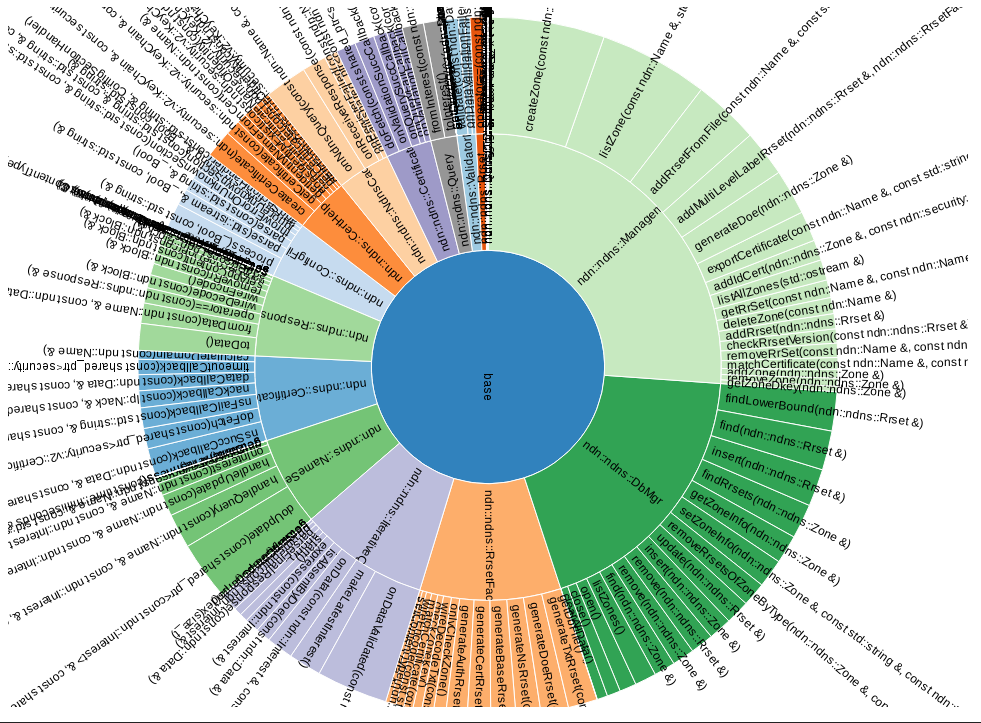
\includegraphics[width=0.5\textwidth]{ndns-sunburst.png}
\caption{NDNS Sunburst Plot}
\label{fig:ndns-suburst}
\end{figure}

\begin{figure}
\centering
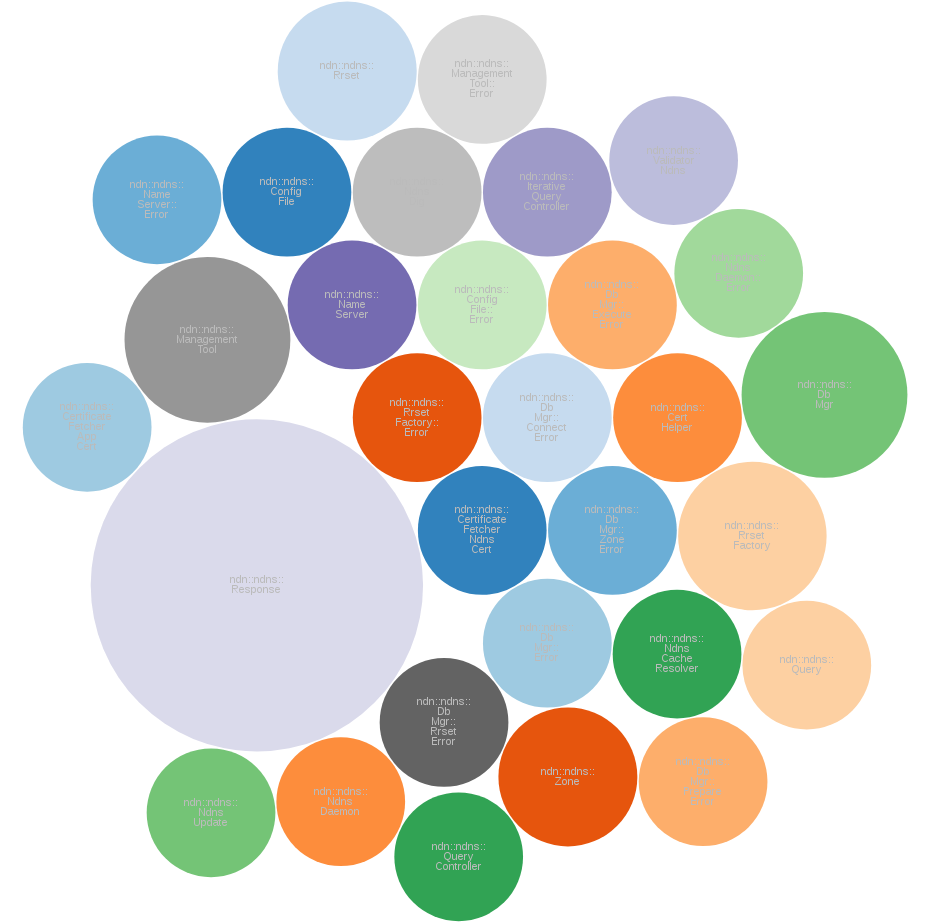
\includegraphics[width=0.5\textwidth]{pagerank.png}
\caption{Page Rank Plot}
\label{fig:pagerank}
\end{figure}

\begin{figure}
\centering
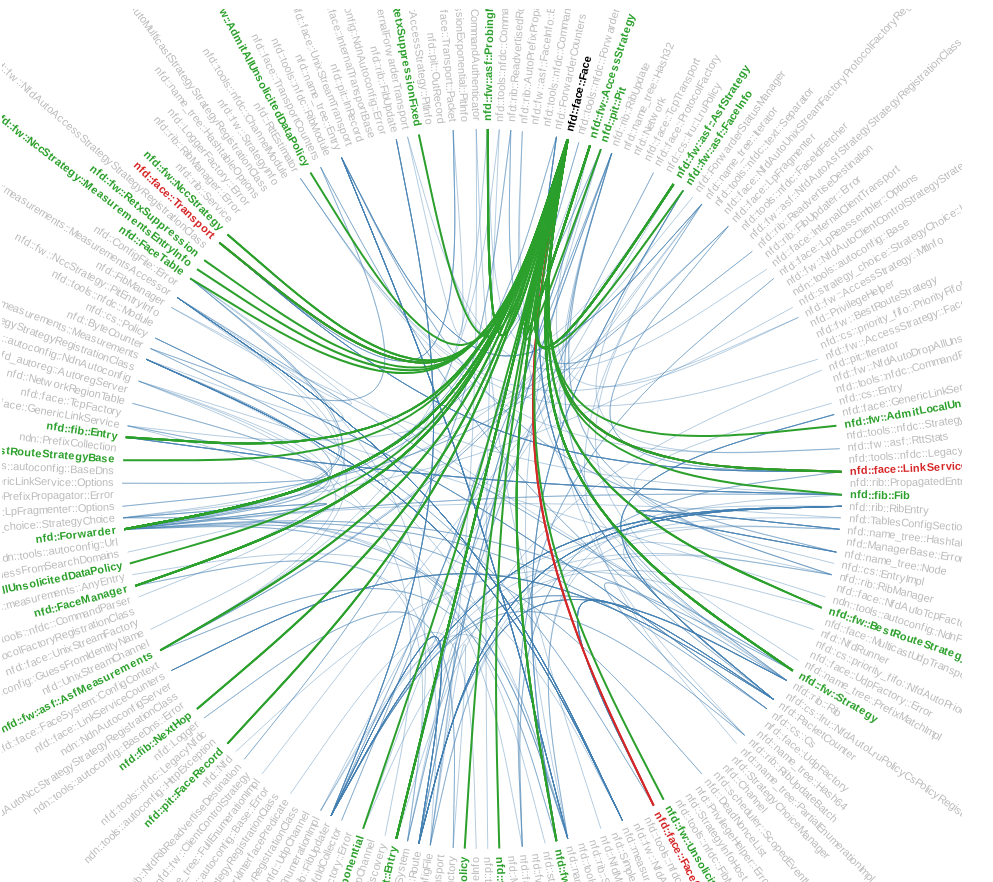
\includegraphics[width=0.5\textwidth]{usage-dependency.png}
\caption{Usage Dependency Plot}
\label{fig:usagedependency}
\end{figure}

\begin{figure}
\centering
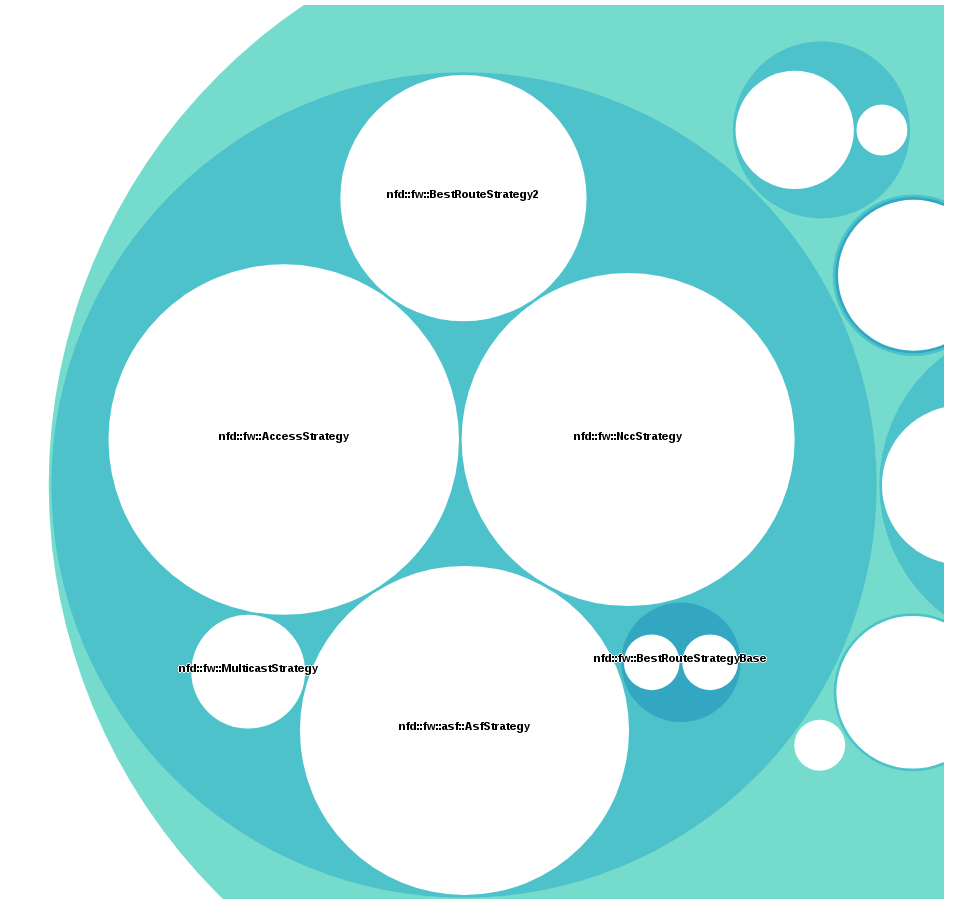
\includegraphics[width=0.5\textwidth]{class-hierachy-zoomed-in.png}
\caption{Class Hierarchy Zoomed In Plot}
\label{fig:class-hierachy-zoomed-in}
\end{figure}

\begin{enumerate}
\item Hierarchy Tree (Fig.~\ref{fig:hierachytree})\\
As the name indicates, the Hierarchy Tree plot reflects the inherited relation of a codebase. Specifically, it allows user to specify whether s/he wants to get the inherited relationship among classes or the methods call relationship. The structure is constructed based on the collapsible tree as each node represents either a class or method. If the node is colored blue, it means the node is collapsible. Users can click on the node to find which class is inherited from the current class or which methods get called. On the other hand, if the node is colored white, it means the bottom level of hierarchy or method call has been reached and no allowance in our tool for a further click.

\begin{figure}
\centering
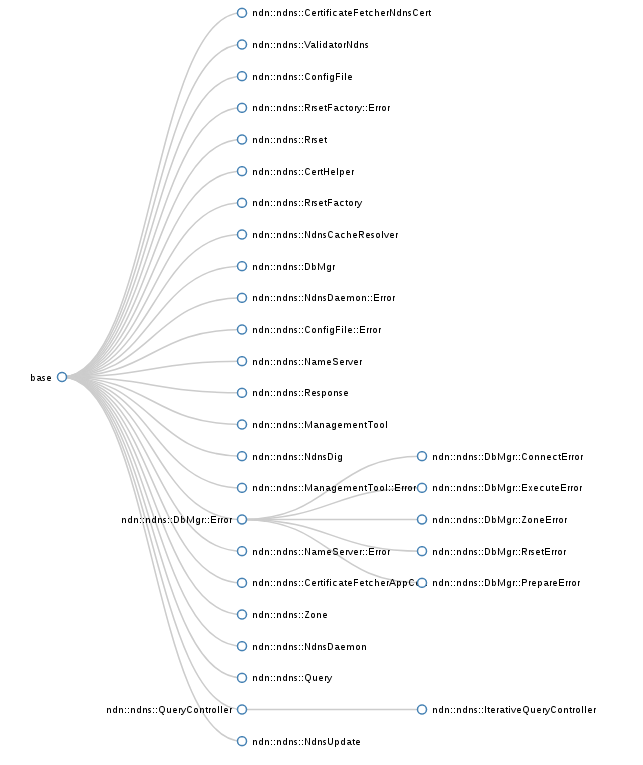
\includegraphics[width=0.5\textwidth]{ndns-hierachy.png}
\caption{NDNS Hierarchy Tree Plot}
\label{fig:hierachytree}
\end{figure}

\vspace{-6pt}
\item Sunburst (Fig.~\ref{fig:ndns-suburst})\\
Sunburst is also a plot to represent the Hierarchy structure. Instead of using the tree representation, it uses "pie chart - like" representation. The advantage of this representation is that it offers not only a direct view of the hierarchy structure, but also provides an explicit percentage of each metric that needs to be measured. The users can select either the inherited relationship or methods call relationship together with the metric; 3 metrics are available in the current version, which are lines of code, number of methods and number of fields. It allows users to click on one portion of the pie chart to get into the class or method if the dimension of it is higher than others in the same circle. To get back to the upper level, users can just click the center of the zoom-in plot.
\vspace{-6pt}
\item Edge Bundling \\
Edge bundling provides information of the inherited relationship and methods call relationship. If the cursor is placed on the words, the color of the edge will tell the relationship between all the related methods. The color green means that this class is a subclass, and is inherited from the class on the other side of the edge. The color red means that this class is inherited from the class on the other side of the edge. As for methods, the color green means that this method is called by the method on the other side of the edge, and the color red means that this method calls the methods on the other side of the edge. This graph is really intuitive for people to understand the relationship between different classes and methods.
\vspace{-6pt}
\item Circle Packing (Fig.~\ref{fig:class-hierachy-zoomed-in}) \\
Circle Packing is another plot to represent the hierarchy structure interactively. Instead of static circles, we made some adaption and enabled the zoomable feature of circles that allows uses to go into a specific class or method to look for details. Inherited relationship and methods call relationship can be chosen as well, and the size of the circles represent the metric that users specify themselves. For example, if lines of code is chosen, then the circle with bigger size / higher radius is the class / method contains more code. By the same token, this visualization feature applies to number of methods and number of fields as well.
\vspace{-6pt}
\item PageRank (Fig.~\ref{fig:pagerank}) \\ 
As an important feature of our project, we conduct the PageRank algorithm based on the usage dependency. After all results convert to the intermediate representation, server iteratively goes through whole list and record all classes in one dictionary. Then we record the times of the class appeared in the usage dependency like method parameters list, field type and etc. After that, the information stored in dictionary include the outClass, inClass and corresponding reference times. Then we put whole dictionary into \emph{Pandas} PageRank tool. As the output of the PageRank tool, it will include all class name and corresponding page range. The output will be presented in bubble graph. We evaluate the usage dependency of each class in the graph. The size of bubble represents the usage as bigger bubble indicates high usage. Since it is easy to extend the result, we can also apply other measurements such as inheriting information.

\end{enumerate}


\section{Evaluation}

To assess the applicability of DUCK in helping developers understand the source codes with different scale of project, under different scenarios, we designed a study aiming to answer the following research questions:
\begin{enumerate}
\item \textbf{RQ1}: Does DUCK help tester understand the source codes? How would they rate the helpfulness of DUCK?
\vspace{-6pt}
\item \textbf{RQ2}: What are the helpful information testers gained by using DUCK in common?
\vspace{-6pt}
\item \textbf{RQ3}: Does interactive figure and query-able visualization address the scalability issue?
\end{enumerate}

\subsection{Experiment Setup}

\textbf{Subject Selection}: To investigate our research questions, we run DUCK on two community-developed C++ open source projects: NDNS and NFD, which are different in scale, the number of developers, and years of development. The detail information is listed in table.\ref{table:examinedProject}. The reason why we choose these two projects is that two of our authors are seasoned developers or authors of them. They have first hand experience on those code and they can answer questions like the importance of class, subjectively.

\begin{table}[]
\centering
\caption{Examined Project}
\label{table:examinedProject}
\begin{tabular}{|l|l|l|l|}
Project & Description & Age & LoC \\
NDNS   & A NDN DNS router & 2 & 8643   \\
NFD & NDN Router Daemon & 4 & 63021                         
\end{tabular}
\end{table}

\textbf{Survey Questions}:a survey of several questions is done by the testers to reflect their understanding on the codebase.  After collecting a reasonable amount of survey results, experienced developers, who are already familiar with the code, will then evaluate the understanding level towards the code base between these two groups by analyzing their answers. We show that the hypothesis in the proposal is confirmed that our visualization tool does help people understanding a new code base.

\textbf{Testers Recruiting}: We asked twenty colleagues(all of them are graduate or PhD students who are now currently studying in CS related major) to do the survey. The majority of the participants have some software development experience, and several students even have some experience in using or designing software visualization tools. We believe their results on the survey can generally reflect their understanding of the code after using DUCK and their opinions and suggestions are valuable for a future version of DUCK.

\subsection{RQ1}
The result of the survey confirmed that DUCK does help testers better understanding the code. For those who have no experience in using or designing software visualization tools, they all like the way DUCK represents the code. Different participants have their own tastes of the plots. For example, one of the tester justifies her reason why she likes Edge Bundling plot. She thinks that DUCK facilitates the understanding of relationships between classes and she can easily understand and intuitively feel how those classes work interactively. What's more, at the end of the concrete question, we asked the testers to self-evaluate their understanding level of the code after using DUCK. The codebase is totally new to everyone before the test, and after experiencing DUCK, the average value is 5.6, which indicates that DUCK can serve as a test water visualization tool for the developers when facing a new system.

\subsection{RQ2}
According to the reasons of testers to justify their choices to the questions, they were all impressed by the attributes DUCK provides to measure the code. One thing we noticed is that, all testers successfully solved our 8-1st question that, "if you want to change the API of ndn::ndns::Validator\\Ndns, which classes you want to inspect?". Testers responded
that they just looked at the usage dependencies graph, which tells them which classes used validatorNdns. Also, for 8-2nd question, testers all provide right answers, by checking the same usage graph, to the question that 'if an exception was thrown in ndns::Zone', which of the following class you want to exterminate? However, as for pageRank graph, some testers found this part confusing, since some iterator classes, which are meaningless in understanding the codes, have higher value than most of the classes.


\subsection{RQ3}
Judging from our results, all testers believe that interactive figure and query-able visualization can effectively help them select the contents they might be interested in NFD project. One thing worthwhile to be mentioned is that many testers commented that interactive figure keeps the golbal view, at the same time, DUCK allows them to zoom in and zoom out the figure, which makes the shift between local and global view. Specifically, not only can the users have a general information of the inherited and interactive relationship, but also detailed information of a certain class or method can be displayed clearly with a signle click of it. On the other hand, many
testers claim that, because that there are so many classes in NFD project, even if they could use iterative figure to zoom-in into the portion they are interested, irrelevant classes degrade their experience of using DUCK. However, when we tell them that they could use query-able visualization feature, to select only the class they want to know, they responded that this feature is very helpful.  


\section{Threats to validity}
We conduct a survey to evaluate the understanding level of testers with a completely new codebase based on the results. Below, we try to explain the threats of validity in our tool.

\textbf{Internal Validity:} To select the participants of the survey, we randomly sent out the survey to undergraduates, graduates and currently CS-related workers with software development experience. Then, we presented them with the codebase which is completely new to them. By manually setting some related questions such as the importance of the methods, dependencies on different classes and hierarchy information of the system, we assumed testers can at least gain some basic high-level ideas about the system after using DUCK. In order to make the result more accurate, we did not choose our testers that already have strong software development experience in the related field, since they might have similar development experience before and their understanding of the codebase might not directly improved from DUCK. 

\textbf{Construct Validity:} We assumed that the results of the survey can show testers' understanding level of the system. Here, we ignored the other causes which are not included in the survey that might also reflect how well testers understand the code. In addition, by designing the survey, we assumed that testers' idea on the system can be extracted from results of this survey, which introduced subjective bias. In terms of evaluation, it is obviously impossible to summarize all the factors that help the testers to understand the system. In this case, we tried to analyze our tool based on the results we obtained on the survey.

\textbf{Conclusion Validity:} In order to evaluate the performance of DUCK, we manually analyzed the surveys and referred the answers from testers to the understanding of the original codebase developers. However, this process inevitably introduced conclusion bias. For example, we assumed that testers understood the code well if they can answer the questions correctly or can mark high on their self-evaluation on their understanding with the help of DUCK, which might not always be convincing.       

\section{conclusion}
It is usually difficult to understand a large codebase, especially for developers who have no development experience on a given codebase. To solve this problem, we designed and implemented DUCK, a powerful visualization tool that can parse the origin codebase and generates interactive results. To our best knowledge, DUCK is the only free and open source visualization tool available right now. We evaluated our tool by using a well-organized codebase called Named-Data Networking (NDN) and a well-designed survey. The evaluation result from the survey shows that DUCK does help developers improve their understanding level towards an unfamiliar codebase. Even for developers who are familiar with the codebase, DUCK can still help them find interesting results in terms of different metrics, or even find potential threats in the code design through DUCK.

\section{future work}
In this paper, a Dynamic Universal Software System Visualization Kit, DUCK is implemented as a powerful tool in helping developers when they are facing a codebase which is completely new to them. After conducting a well-designed survey, we analyzed participants understanding level of the codebase after using DUCK. The result confirmed that DUCK actually helps the developers better understanding the code. However, there are still some limitations on DUCK, also we received some suggestions and future improvements on DUCK. We list them in detail and hope for a new version of DUCK that can finish these tasks and better serve as a outstanding software visualization tool in the future. 
\begin{enumerate}
\item The font of plots can be clearer when the codebase is larger.
\vspace{-6pt}
\item No overlapping on the class names.
\vspace{-6pt}
\item More attributes such as most called method can be added to better represent the codebase.
\vspace{-6pt}
\item When clicking on certain class or method for more information, DUCK should provide a better interaction with the users and help locate it if necessary.
\end{enumerate}

%% \footnote{This is the second footnote.  It
%% starts a series of three footnotes that add nothing
%% informational, but just give an idea of how footnotes work
%% and look. It is a wordy one, just so you see
%% how a longish one plays out.}

%% \cite{Lamport:LaTeX}

%
% The following two commands are all you need in the
% initial runs of your .tex file to
% produce the bibliography for the citations in your paper.
\bibliographystyle{abbrv}
\bibliography{sigproc}  % sigproc.bib is the name of the Bibliography in this case
% You must have a proper ".bib" file
%  and remember to run:
% latex bibtex latex latex
% to resolve all references
%
% ACM needs 'a single self-contained file'!
%
%APPENDICES are optional
%\balancecolumns
\appendix
%Appendix A

\section{Individual Contribution}
\label{IndivContri}
In this project, we have very clear division of work. Yumin is in charge of the implementation of a parser-like analysis tool, which supports C++ currently. As introduced in Section.\ref{static}. Yukai is in charge of generating the intermediate representation of the data generated from Yumin. He is also in charge of developing the query-able attribute processor. Shan and Yuling is in charge of the User Interface design of our system and the exploration of different plotters. They also determine the type of metrics that is important of analyzing the codebase and implement the perfect plot to represent such information. Cong is mainly in charge of the empirical study part. He designs the survey questions, and enroll a lot of participants to take the survey. Then, he collects all the surveys and analyzes the survey results. 

\section{Intermediate Representation Example}
\label{IReg}

\begin{lstlisting}[language=json,firstnumber=1]
{  
   "classes":{  
      "class ndn::ndns::CertificateFetcherAppCert":{
      "fields": {
        "m_validator": "class ndn::ndns::ValidatorNdns",
        "m_face": "class ndn::Face"
      },
      "methods": {
        "doFetch(CertificateRequest &, ValidationState &, ValidationContinuation &)": {
          "return_type": "void",
          "linesOfCode": 22,
          "parameter": {
            "continueValidation": "class ValidationContinuation",
            "state": "class shared_ptr<security::v2::ValidationState>",
            "certRequest": "class shared_ptr<security::v2::CertificateRequest>"
          },
          "calling-function": [],
          "run-time-invokes": 0
        }
      },
      "base_list": [
        "security::v2::CertificateFetcher"
      ]
    }
   }
}
\end{lstlisting}
\section{Investigation On Other Visualization Tool}

\begin{figure}
\centering
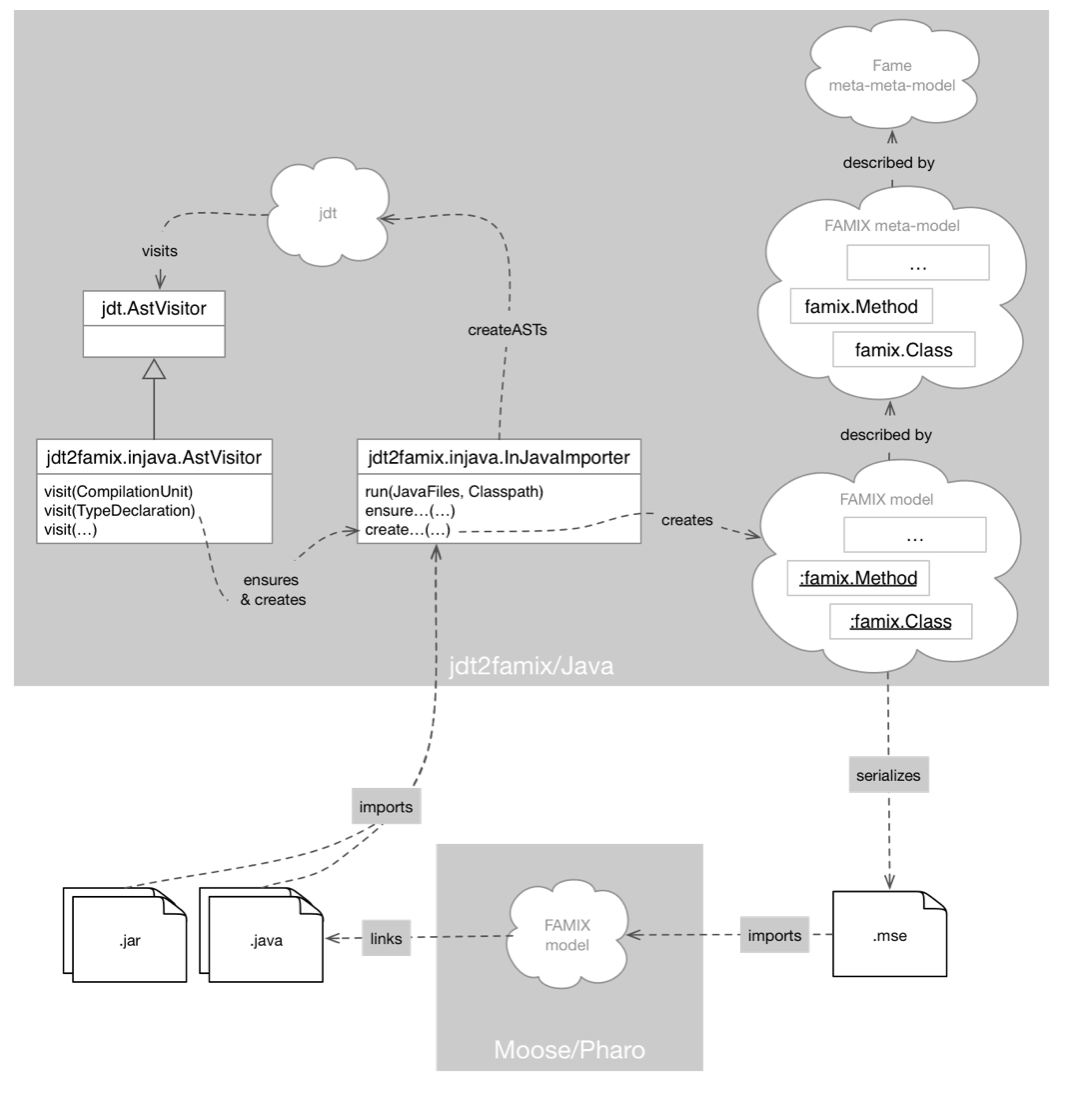
\includegraphics[width=0.5\textwidth]{eva1.png}
\caption{Structure of jdt2famix and interaction with Moose}
\label{fig:structure of jdt2famix and interaction with Moose}
\end{figure}

Moose is a platform for software and data analysis. It helps programmers craft custom analyses cheaply. It's based on Pharo. Especially for Java repository, the external tool, jdt2famix  (Fig.~\ref{fig:structure of jdt2famix and interaction with Moose}), is provided. It offers the mechanism for producing MSE files out of Java code. It is based on JDT Core and Fame for Java, and it requires Java 8. The baseline study has been conducted on previous work on software visualization. On one of the reference paper, a version of Polymetric Views is implemented on the demo data of the source of spring-core, which is part of the Spring Framework.

Moose is a platform for expressing analyses of software systems and of data in general. Its main goal is to assist and enable a human in the process of understanding large amounts of data.

The analysis process is customizable. The job of dedicated engines is to help the engineer craft new importers, models and analyses.
The input is always some piece of data. By data, we understand all sorts of structures that contain objects, properties and relations. For example, data can be a software system written in Java. Or it can be a set of configuration files written in XML. Or it can be some meta-data about your system. Or it can be a text file.
This data is loaded in Moose via importers. You can import data from various sources and in various formats. For example, you can import the structure of software systems either through internal importers (e.g., for Smalltalk code, XML, JSON, MSE), or through external ones (e.g., Java).
The importing of data can be perceived as a rather unexciting step, but it is a necessary one. Once imported, the data is stored into models. This is where things get more interesting because on top of these models you can start performing various kinds of analyses.
What do we mean by analyses? Metrics, queries, interactive visualizations etc. There a multitude of basic services like these provided by default. These tools can be applied interactively, and can be combined to produce more complex analyses such as: computation of dependency cycles, detection of high level design problems, identification of exceptional entities and so on. A key concept is that the results obtained after applying a specific analysis are fed back into the model and are available for further analysis. This enables an iterative process through which the analysis is built and refined gradually.
Here we test Moose in an example as a case study. In this case, we take ArgoUML, an open-source Java project.

It also provides 'select' option to group the source code with same attributes. For example, at this point, we are only interested in the deprecated classes, so let's select only those are annotated with 'Deprecated'.

By exploring the view of selected classes, we can visualize them in an interactive picture of nodes, which can reveal the details of the actual class to the right.

There are several options provided to visualize the source code, for example, by distinguishing between the deprecated and the non-deprecated classes, or by checking the dependencies between classes, or by arranging the nodes in a clearer pattern (Fig.~\ref{fig:Different views for visualization of Moose I}).

\begin{figure}
\centering
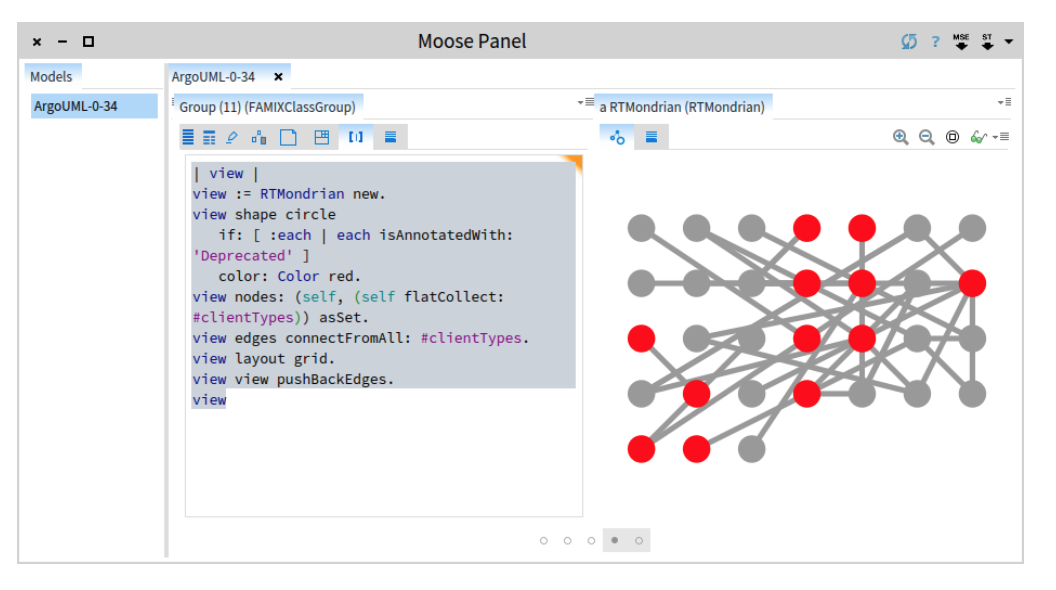
\includegraphics[width=0.5\textwidth]{eva6.png}
\caption{Different views for visualization of Moose I}
\label{fig:Different views for visualization of Moose I}
\end{figure}

\end{document}
